
\chapter{Hybrid Finite/Boundary Element Method}
\label{sec:hybr-finit-elem}
The hybrid finite/boundary element method works similarly to the normal finite element method except that one or more sub-regions are mapped onto their boundary \cite{Rammohan2002}.
The main advantage of this is that we reduce the dimensionality of these sub-regions one since we only have to solve equations on the boundary instead of the entire space.
In our case this is likely to give an advantage over a pure finite element method since we no longer need to mesh a long way outside the magnetic domain to accurately account for the effect of the external region. Also other methods for dealing with infinite domains can often give additional errors due to the truncation of the external domain.\cite{Bottauscio2008}

On the downside this mapping typically results in a dense matrix after discretisation, to which we cannot apply sparse matrix techniques.
Also the integrals that need to be computed may involve singularities, which introduce additional complications and may reduce accuracy or increase computation time.

Note that the derivation for this hybrid method comes from potential theory, rather than the boundary integral formulation usually used to construct the standard boundary element method.

\section{Derivation of the continuous problem}
\label{sec:bem-derivation}

\subsection{Background of the Method}
\label{sec:basic-method}
We want to use the boundary element method in the calculation of the magnetostatic scalar potential $\phim$, ($\hms = - \nabla \phim$), in the infinite region outside of a magnetic body.
Using the boundary element method directly, however, would require the solution of dense matrix equations for the entire problem.

We can circumvent this problem by splitting the potential into two parts $\phim = \phione + \phitwo$ in such a way that $\phione$ can be calculated the magnetic region(s) using only the finite element method.
We then have some conditions on $\phitwo$ that must be satisfied to give the correct total potential in $\magd$ and on $\boundd$, but, in order to solve for $\phitwo$ in the magnetic domain, we still need to find the boundary conditions (on the edge of the magnetic domain).
So we choose a charge distribution on the boundary that satisfies all the conditions on $\phione$ and $\phitwo$.
We can then solve for $\phitwo$ on the boundary using similar techniques to those used in the boundary element method.
Finally we apply the finite element method to find $\phitwo$ inside the magnetic region $\magd$.

By the uniqueness of solution for Poisson's equation with Dirichlet and/or Neumann boundary conditions we know that the field $ \hms = \nabla \phim$  constructed by the above steps is \emph{the} magnetostatic field.\footnote{To see this take the difference of two solutions of Poisson's equation: $\phi = \psi_1 - \psi_2$. Then using identity \eqref{eq:20}, the linearity of Poisson's equation and the divergence theorem we obtain $\int_S \phi \nabla \phi \cdot d \mathbf{S} = \int_V (\nabla \phi)^2 dV$. Applying Dirichlet, Neumann or mixed boundary conditions shows that the boundary integral is zero and hence $\nabla \phi = 0$.}

\subsection{Problem Description}
\label{sec:problem-description}
Let $\phim^\inte$ be the value of $\phim$ (with subscripts as appropriate) close to the boundary $\boundd$ and just inside the magnetic domain  and $\phim^\exte$ the value of $\phim$ just outside the magnetic domain\footnote{More precisely $\phim^\inte(\xv) = \lim_{\xv \rightarrow \boundd} \phim(\xv)$ from inside the magnetic domain, $\phim^\exte(\xv) = \lim_{\xv \rightarrow \boundd} \phim(\xv)$ from outside the magnetic domain.} (see \autoref{fig:BEM-geometry}).

We have the following \emph{physical} conditions\footnote{Equations~\eqref{eq:2}-\eqref{eqn:phibound} come from the definition of $\phim$, requirement for finite total energy, $\Bv^\text{int} \cdot \nv = \Bv^\text{ext} \cdot \nv$ and ??ds respectively.} on the total magnetostatic potential $\phim$:
\begin{equation}
  \lap \phim(\xv) = \nabla \cdot \mv(\xv) \qquad \forall \xv \in \magd \cup \extd,
  \label{eq:2}
\end{equation}
\begin{equation}
  \phim(\xv) \rightarrow 0 \qquad \text{ as } \abs{\xv} \rightarrow \infty,
\end{equation}
\begin{equation}
  \pd{\phim^\inte(\xv)}{\nv} - \pd{\phim^\exte(\xv)}{\nv} = \mv \cdot \nv \qquad \xv \in \boundd,
  \label{eqn:dphibound}
\end{equation}
\begin{equation}
  \phim^\inte(\xv) - \phim^\exte(\xv)  = 0 \qquad \xv \in \boundd.
  \label{eqn:phibound}
\end{equation}
Note that equations~\eqref{eqn:dphibound} and \eqref{eqn:phibound} imply continuity but not smoothness of the magnetic potential $\phim$ across $\boundd$. This is due to surface magnetic charges.

We choose $\phione$ to satisfy:
\begin{equation}
  \phim(\xv) = \phione(\xv) + \phitwo(\xv) \qquad \forall \xv \in \fulld,
  \label{eq:21}
\end{equation}
\begin{equation}
  \lap \phione(\xv) = \nabla \cdot \mv(\xv) \qquad \xv \in \magd,
  \label{eq:1}
\end{equation}
\begin{equation}
  \pd{\phione^\inte(\xv)}{\nv} = \mv \cdot \nv \qquad \xv \in \boundd,
  \label{eqn:dphionebound}
\end{equation}
\begin{equation}
  \phione(\xv) = 0 \qquad \xv \in \extd.
  \label{eqn:phioneoutside}
\end{equation}
Note that equations~\eqref{eq:1} and \eqref{eqn:dphionebound} give a self contained Poisson Neumann problem for $\phione \in \magd \cup \boundd$.

The equations~\eqref{eq:2} to \eqref{eqn:phibound} for $\phim$ combined with equations~\eqref{eq:21} to \eqref{eqn:phioneoutside} for $\phione$ give a number of conditions on $\phitwo$ must satisfy. Since the Laplacian operator is linear, \ie $\lap \phim = \lap \phione + \lap \phitwo$, from \eqref{eq:2} and \eqref{eq:1} it follows that
\begin{equation}
  \label{eq:8}
  \lap \phitwo(\xv) = 0 \qquad \forall \xv \in \fulld.
\end{equation}

Equation~\eqref{eqn:phioneoutside} implies that $\pd{\phione^\exte(\xv)}{\nv} = 0$. Combining this with equations \eqref{eqn:dphionebound} and \eqref{eqn:dphibound} gives
\begin{equation}
  \label{eq:5}
  \pd{\phitwo^\inte(\xv)}{\nv} - \pd{\phitwo^\exte(\xv)}{\nv} = 0.
\end{equation}

Finally from equations \eqref{eqn:phibound}, \eqref{eq:21} and \eqref{eqn:phioneoutside} we have
\begin{equation*}
  \phione^\inte - \phione^\exte + \phitwo^\inte - \phitwo^\exte = 0,
\end{equation*}
\begin{equation}
  \phitwo^\inte - \phitwo^\exte = - \phione^\inte.
\label{eq:4}
\end{equation}

\begin{figure}
  \center
  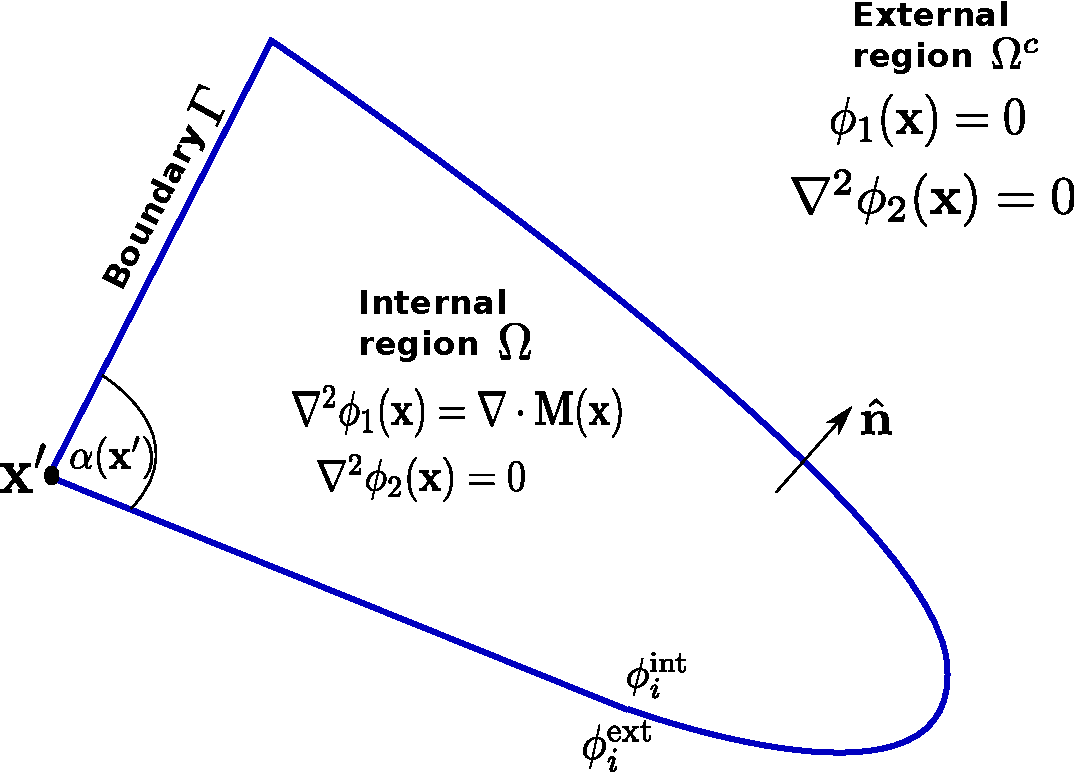
\includegraphics[width=0.75\textwidth]{./images/BEM-geometry}
  % \begin{tikzpicture}

  %   % Main nodes and some labels
  %   \node[label=below:$\xv'$] (a) at (-2,-2) {};
  %   \node (b) at (-2,2) {};
  %   \node[label=right:\Large{$\boundd$}] (c) at (5,0) {};

  %   % Draw main shape of magnetic domain
  %   \draw [line width=0.5mm,draw=solidblue,fill=paleblue] (a.north) to [bend right=71] (c) to (b.south);
  %   \draw [line width=0.5mm,draw=solidblue] (a) to (b);
  %   \draw (a.north) circle(1mm) [fill=black] {};

  %   % More labels
  %   \node (center) at (1,0) {\Large{Magnetic domain $\magd$}};
  %   \node(external) at (8,3) {\Large{External region $\extd$}};
  % \end{tikzpicture}

  \caption{A 2D representation of the geometry showing the labels used in this section. The point $\xv'$ is a singular point of the boundary $\boundd$, the angle $\alpha(\xv')$ is as shown.}
  \label{fig:BEM-geometry}
\end{figure}

\subsection{Double Layer Potentials}
\label{sec:double-layer-potent}
A double layer potential can be thought of as the potential due to a layer of dipoles of magnitude $\mu(\xv)$ in direction $\nv$ over the surface $S$.\cite{Sternberg1946} We will demonstrate that we can use a double layer potential to calculate $\phitwo^\inte$ in terms of $\phione^\inte$.

The double layer potential at a point $\xv \in \real^d$ is defined as \cite{eom_double_layer_potential}
\begin{equation}
  \label{eq:3}
  \phim(\xv) = \int_{S} \mu(\yv) \pd{\Green}{\nv(\yv)} \d \yv,
\end{equation}
where $G$ is the Green's function for a Laplacian operator.
For $d=2$
\[ \Green = \dfrac{-1}{2\pi}\ln(\abs{\xv - \yv}), \]
and for $d=3$
\begin{equation} \Green = \dfrac{-1}{4 \pi} \dfrac{1}{\abs{\xv - \yv}}.
  \label{eqn:greenslaplacian3d}
\end{equation}


We have the following results from potential theory:\cite{Sternberg1946}
\begin{enumerate}
\item The double layer potential satisfies Laplace's equation $\lap \phi = 0$ (in other words the double layer potential is harmonic).% pages ?

\item The double layer potential undergoes a jump of $\mu(\xv)$ moving in the direction $\nv$ across a smooth surface $S$, \ie
  \begin{equation}
    \label{eq:15}
    \phim^\inte(\xv) - \phim^\exte(\xv) = \mu(\xv).
  \end{equation}
% pages 136-140

\item For $\xv \in S$ the following relationship holds
  \begin{equation}
    \phim^\inte(\xv) = (1 - \frac{\alpha(\xv)}{\alpha_{\text{max}}}) \mu(\xv) + \phim(\xv),
    \label{eq:22}
  \end{equation}
  where $\alpha(\xv)$ is the angle (or solid angle) in two (or three) dimensions subtended by the domain at $\xv$ and
\begin{equation*}
  \alpha_{\text{max}} =
  \begin{cases}
    2 \pi & \text{if } d=2 \\
    4 \pi & \text{if } d=3.
  \end{cases}\label{eq:16}
\end{equation*}
Note that $\alpha(\xv)$ is the angle at the exact point $\xv$, when the surface at $\xv$ is a Lyapunov surface (\ie not a sharp corner) $\frac{\alpha(\xv)}{\alpha_{\text{max}}}$ reduces to a factor of $1/2$. We write $\gamma(\xv) = \frac{\alpha(\xv)}{\alpha_{\text{max}}}$ for simplicity.
 % pages 137-139, page 155 for 2d

\item If $\mu$ is continuous and has continuous first and second derivatives along the boundary (\ie $\mu(\xv) \in C^2[S]$) then the limits $\pd{\phim^\inte(\xv)}{\nv}$ and $\pd{\phim^\exte(\xv)}{\nv}$ exist and are equal. % pages 145-153.

\end{enumerate}

Some notes on the derivation of the above results in Sternberg 1946\cite{Sternberg1946}:
\begin{itemize}
\item Some derivations of the results above rely on the surface being a ``Lyapunov surface'' which imposes a number of smoothness conditions, in particular excluding surfaces with corners.
The proofs given in Sternberg allow a finite number of sharp corners, \ie a polygonal domain.
\item Our potentials are a factor of $\frac{-1}{4 \pi}$ different from those in the reference. Also our $\phim^\inte$ and $\phim^\exte$ definitions correspond respectively to $\phim^-$ and $\phim^+$ in the book.
\end{itemize}

\subsection{Application to Magnetostatic Calculations}
\label{sec:appl-magn-calc}

From \autoref{sec:double-layer-potent} we can see that conditions \eqref{eq:8}, \eqref{eq:5} and \eqref{eq:4} on $\phitwo$ are satisfied by a double layer potential with magnitude
\begin{equation}
  \label{eq:24}
  \mu(\xv) = - \phione^\inte(\xv).
\end{equation}

By the uniqueness of solution for Poisson's equation this gives us, up to an additive constant, the only solution for $\phitwo(\xv)$ in the external region.
This is good enough for a potential since it is only used in $\hms(\xv) = - \nabla \phim(\xv)$ so addition of a constant has no effect.

From equations~\eqref{eq:3}, \eqref{eq:22} and \eqref{eq:24} we have:
\begin{equation}
  \label{eq:6}
  \phitwo^\inte(\xv) =  \big(\gamma(\xv) - 1 \big) \phione^\inte(\xv)
  - \int_{\boundd} \phione^\inte(\yv) \pd{\Green}{\nv(\yv)} \d \yv.
\end{equation}
After substituting in our definition for the three dimensional Green's function \eqref{eqn:greenslaplacian3d} we obtain the same equation as given by Koehler \cite{Koehler1997}.
Similar equations are solved when using the standard boundary element method, hence the name.

Also note that $\phim = \phione + \phitwo$ everywhere and so
\begin{align}
  \label{eq:18}
  \phim^\inte(\xv) &= \bm \big[ \phione^\inte(\xv) \big] \\
  &= \gamma(\xv) \phione^\inte(\xv)
  - \int_{\boundd} \phione^\inte(\yv) \pd{\Green}{\nv(\yv)} \d \yv. \notag
\end{align}

Either equation~\eqref{eq:6} or \eqref{eq:18} can be used to give boundary conditions for $\phitwo \in \magd$ or $\phim \in \magd$ respectively. We will proceed using equation~\eqref{eq:18} for simplicity since it eliminates $\phitwo$ from later calculations.

Hence, given the solution for $\mv(\xv) \in \magd$ the complete continuous problem is
 \begin{subequations}
   \label{eq:phi-bem-continuous}
   \begin{align}
     \label{eq:phim-bem-continuous}
     \lap \phim(\xv) &= \div \mv(\xv) \quad & \xv \in \magd, \\
     \label{eq:phi1-bem-continuous}
     \lap \phione(\xv) &= \div \mv(\xv)    & \xv \in \magd,
   \end{align}
 \end{subequations}
with boundary conditions
 \begin{subequations}
   \label{eq:phi-bem-continuous-bc}
   \begin{align}
     \label{eq:phim-bem-continuous-bc}
     \phim(\xv) &= \bm \big[ \phione(\xv) \big]      & \xv \in \boundd, \\
     \label{eq:phi1-bem-continuous-bc}
       \pd{\phione(\xv)}{\nv} &= \mv \cdot \nv  & \xv \in \boundd.
   \end{align}
 \end{subequations}
Here we have dropped the distinction between $\inte$ and $\exte$ since all exterior values have been eliminated.


\section{Discretisation}
\label{sec:discretisation}

The bulk equations~\eqref{eq:phi-bem-continuous} and the boundary condition on $\phione$, equation~\eqref{eq:phi1-bem-continuous-bc}, are identical to those discussed in \autoref{sec:llg-initial-equations}.
As such the weak residual form, discretisation and Jacobian calculations are identical for these equations.
Therefore all that remains to be discretised is the operator $\bm$. We let
\begin{equation}
  \phim = \sum_\ibasis \phim_{\ibasis} \tbf_{\text{m},\ibasis}(\xv),
  \qquad
  \phione = \sum_\ibasisb \phione_{\ibasisb} \tbf_{1,\ibasisb}(\xv),
  \label{eq:25}
\end{equation}
where $\tbf_\ibasis(\xv_\ibasisb) = \delta_{\ibasis \ibasisb}$ on the boundary nodes and is linearly interpolated from $\tbf_\ibasis = 1$ at $\xv_\ibasis$ to $\tbf_\ibasis = 0$ at neighbouring nodes.

Substituting equations~\eqref{eq:25} into \eqref{eq:18} we have
\begin{equation*}
  \sum_\ibasis \phim_{\ibasis} \tbf_{\text{m},\ibasis}(\xv) =
  - \int_{\boundd} \sum_\ibasisb \phione_{\ibasisb} \tbf_{1,\ibasisb}(\yv)
  \pd{\Green}{\nv(\yv)} \d \yv
  \quad + \gamma(\xv) \sum_\ibasisb \phione_{\ibasisb} \tbf_{1,\ibasisb}(\xv).
\end{equation*}

To get the value of $\phim$ at node $\ibasisc$ we choose $\xv = \xv_\ibasisc$. Then using the property $\tbf_\ibasis(\xv_\ibasisc) = \delta_{\ibasis \ibasisc}$ and replacing $\ibasisc$ by $\ibasis$ we have
\begin{equation}
  \phim_{\ibasis} =
  - \int_{\boundd_\ibasisb} \sum_\ibasisb \phione_{\ibasisb} \tbf_{1,\ibasisb}(\yv)
  \pd{\Green[\ibasis]}{\nv(\yv)} \d \yv
  \quad + \gamma(\xv_\ibasis) \phione_{\ibasis},
  \label{eq:colocation}
\end{equation}
where ${\boundd_\ibasisb}$ is the region where $\tbf_{1,\ibasisb} \neq 0$, \ie the elements which contain node $\ibasisb$.

Finally, since the integrands are continuous functions ??ds citation needed, we can move the sum outside the integral leaving
\begin{equation}
  \phim_{\ibasis} =
  - \sum_\ibasisb \phione_{\ibasisb} \Big[ \int_{\boundd_\ibasisb} \tbf_{1,\ibasisb}(\yv)
  \pd{\Green[\ibasis]}{\nv(\yv)} \d \yv \Big]
  \quad + \gamma(\xv_\ibasis) \phione_{\ibasis}.
\label{eq:27}
\end{equation}
Notice that the expression inside the square brackets is independent of all the potentials: it depends only on the geometry and so can be pre-calculated and stored in many cases.

So equation~\eqref{eq:27} gives $\phim$ at a boundary node in terms of a sum of geometric factors multiplied by $\phione$ at each boundary node.
In other words, this is a dense matrix multiplication by a pre-computed matrix giving $\phim$ at all the boundary nodes in terms of $\phione$ at all boundary nodes:
\begin{equation}
  \label{eq:10}
  \phim_\ibasis = \bm_{\ibasis,\ibasisb} \cdot \phione_{\ibasisb},
\end{equation}
where
\begin{equation}
  \label{eq:17}
  \bm_{\ibasis\ibasisb} = - \int_{\boundd_\ibasisb} \tbf_{1,\ibasisb}(\yv) \pd{\Green[\ibasis]}{\nv(\yv)} \d \yv
  \quad + \gamma(\xv_\ibasis)\delta_{\ibasis\ibasisb}.
\end{equation}


% ??ds wrong place for this discussion and not sure if integral is really singular or not due to the n.r term...
%Note that although this integral appears at first glance to be singular when the node $\xv_\ibasis$ is within $\boundd_\ibasisb$ (the line segment or section of surface being integrated over)
%A benefit of this is that the matrix is always well conditioned because the largest terms are near the singularity and hence near the diagonal elements $\ibasisb = \ibasis$.
%However the singularity can cause difficulties in the evaluation of the affected integrals.
%Methods to overcome these difficulties are discussed in the next section.

We now convert the normal derivative of the Green's function into a more tangible form.
In 3D
\begin{equation}
  \label{eq:11}
  \pd{\Green}{\nv} = \frac{-1}{4 \pi} \pd{}{\nv} \Gthreed = \frac{-1}{4 \pi} \nv \cdot \nabla \Big( \Gthreed \Big).
\end{equation}
Converting to spherical coordinates with the origin at $\xv$ ($r = \abs{\yv - \xv}$, $\ruv = \frac{\yv - \xv}{r}$) we have\footnote{In spherical polar coordinates $\nabla = \ruv \pd{}{r} +  \phiv \frac{1}{r} \pd{}{\phi} + \thetav \frac{1}{r \sin \theta} \pd{}{\theta}$. Obviously $\frac{1}{r}$ has no angular dependence so only the derivative with respect to $r$ is non-zero.}
\begin{equation}
  \label{eq:12}
  \pd{G(r)}{\nv} = \frac{-1}{4 \pi} \nv \cdot \ruv \pd{}{r} \Big( \frac{1}{r} \Big)
  = \frac{+1}{4 \pi}  \frac{\nv \cdot \ruv}{r^2},
\end{equation}
\begin{equation}
  \label{eq:13}
  \pd{\Green}{\nv} = \frac{\nv \cdot (\yv - \xv)}{4 \pi \abs{\yv - \xv} ^2} .
\end{equation}
Similarly in 2D we find
\begin{equation}
  \label{eq:14}
  \pd{\Green}{\nv} = \frac{-1}{2 \pi} \pd{}{\nv} (\Gtwod) = \frac{\nv \cdot (\yv - \xv)}{2 \pi \abs{\yv - \xv}}.
\end{equation}

So the discretised boundary element matrix in $d=2,3$ dimensions is
\begin{equation}
  \label{eq:19}
  \bm_{\ibasis\ibasisb} =\frac{-1}{2^{(d-1)} \pi} \int_{\boundd_\ibasisb} \tbf_{1,\ibasisb}(\yv) \frac{\nv(\yv) \cdot (\yv - \xv_\ibasis)}{\abs{\yv - \xv_\ibasis} ^{d-1}} \d \yv
   \quad + \gamma(\xv_\ibasis)\delta_{\ibasisb\ibasis}.
\end{equation}
We denote the integral in this equation by $I_\bm$.

\subsection{Discretisation Approaches: Co-location vs Galerkin}

In deriving equation~\eqref{eq:colocation} we used a co-location approach rather than the Galerkin approach used in our FEM method.
The reason for this choice is that a Galerkin discretisation would lead to a double integral over the boundary, which would probably be more difficult to calculate.

Not sure what effect this has, if any, on the stability or accuracy of the scheme...

\section{Evaluation of the discrete boundary operator}
\label{sec:calc-integr-i_bm}

\section{Singularity of the main integral}
\label{sec:bem-singularity}

Another factor that should be considered is the apparent singularity in the integral $I_\bm$ when integrating over an element containing the source point $\xv_\ibasis$. There are two distinct cases to look at here: flat elements and curvilinear elements.

In the case of flat elements if $\xv_\ibasisb$ is within the element being integrated over then we have
\begin{equation}
  \label{eq:7}
  \nv(\yv) \cdot \ruv_{\xv_{\ibasis} \rightarrow \yv} \equiv 0 \quad \forall \yv \in \text{element}.
\end{equation}
So the integral is zero and the singularity is avoided. Unfortunately for neighbouring elements this is not necessarily true--in particular elements at a sharp corner may be very close to a node where $\nv(\yv) \cdot \ruv_{\xv_{\ibasis} \rightarrow \yv} \neq 0$ resulting in a near-singular integral.

For curvilinear elements we no longer have the nice property that any potentially singular elements are automatically zero. However it can be shown that for reasonably shaped elements ??ds citation needed! there are still no real singular integrals only near-singular ones. This is due to the fact that $\nv(\yv) \cdot \ruv_{\xv_{\ibasis} \rightarrow \yv}$ tends to zero ``faster'' than $\abs{\yv - \xv_\ibasis}^2$ so the limit of the ratio as $\yv \rightarrow \xv_\ibasis$ is zero. In fact integrals like this are routinely evaluated in standard boundary element methods ??ds citation needed.


\subsection{Corner Singularities}

Have to handle calculation of angles/solid angles $\gamma(\xv)$ somehow.

So far I've just assumed the information will be provided

Inderpretations: only count ``real'' sharp corners (\ie sphere has no corners) vs include all element corners (\ie sphere has sharp corners at every element join).


\subsection{Analytical solutions}

??ds you need to thoroughly check the maths in this section at least once more

For linear shape functions and triangular elements an exact analytical solution for the singular integral $I_G$ was given by Lindholm \cite[App. B]{Lindholm1984}\footnote{Note: Lindholm's definition of the 3d Green's function is a factor of -1 different to ours.}, the original derivation is due to Collie\cite{Collie1976}. 
Combining equations (2) and (3) from \cite{Lindholm1984} with equation~\eqref{eq:13} and using our notation for positions, we see that Lindholm's $L$ operator is
\begin{equation}
  \begin{aligned}
    L[U] &= \frac{-1}{4 \pi}\int_\boundd U(\yv) \frac{\nv(\yv) \cdot (\yv -
      \xv)}{\abs{\xv - \yv}^2}
    \d\yv, \\
    &= -G[U] + \gamma(\xv) U(\xv).
  \end{aligned}
\end{equation}
So $L[\tbf_{1,\ibasisb}]$ integrated over the surface triangle $\boundd_\ibasisb$ with $\xv = \xv_\ibasis$ corresponds exactly to the integral $I_{G,i,j}$ required in the calculation of $G_{i,j}$\footnote{The minus sign from the different definitions of the Green's function has cancelled with the minus sign from the fact that we are interested in calculating $-1$ times the operator.}.

To clearly see the equivalence between the discretised operators we need to go through both discretisations simultaneously.
Ignoring sharp corners we have that
\begin{equation}
  \begin{aligned}
    \phim(\xv) = G[\phione](\xv) &= -L[\phione](\xv), \\
    %
    \sum_{n} \phim_n \tbf_n(\xv) 
    &= - \sum_{\tri=1}^{N_\tri} \sum_{i=1}^{3} L_{\tri,i}(\xv) \phione_{\tri,i}, 
    \quad\quad&\text{expand}\\
    % 
    \sum_{n} \phim_n \tbf_n(\xv) 
    &= - \sum_{\tri=1}^{N_\tri} \sum_n L_{\tri,n}(\xv) \phione_n, 
    &\text{equivalent to sum over all nodes--local support}\\
    % 
    \phim_k &= - \sum_{\tri=1}^{N_\tri} \sum_n L_{\tri,n}(\xv_k) \phione_n, 
    &\text{use $\tbf_n(\xv_k) = \delta_{nk}$}\\
    % 
    \phim_k &= \sum_n \bigs{\sum_{\tri=1}^{N_\tri} -L_{\tri,n}(\xv_k)} \phione_n, 
    &\text{reorder}\\
    %
    \phim_k &= \sum_n \bigs{\sum_{\tri \in \text{around}(n)} -L_{\tri,n}(\xv_k)} \phione_n,
    &\text{reduce elements to sum over--local support again}\\
    %
    &= \sum_n G_{k,n} \phione_n. 
    &\text{equation~\eqref{eq:10}}
  \end{aligned}
\end{equation}
Therefore 
\begin{equation}
  IG_{i,j} = \sum_{\tri \in \text{around}(j)} L_{\tri,k}(\xv_i),
\end{equation}
where $k$ is the index of node $j$ within triangle $\tri$.

Let
\begin{equation}
  \begin{aligned}
    \rv_k(\xv) &= \zv_k - \xv, &\quad \text{(vector from triangle node $k$ to $\xv$)} \\
    \sv_k &= \zv_{k+1} - \zv_k, & \text{(vector along an edge of the triangle)} \\
  \end{aligned}
\end{equation}
and let $\hat{\sv}$, $\hat{\rv}$ be the equivalent unit vectors.
Hence using the third (un-numbered) equation in appendix B of \cite{Lindholm1984}, converting to our notation and substituting in values from the rest of appendix B where practical we have
\begin{equation}
  \begin{aligned}
    \label{eq:analytic-bem-integral}
    I_{G,i,j} &= \sum_{\tri \in \text{around}(j)} \frac{\abs{\sv_{k+1}}}{8 \pi A_\tri} \bigb{
      \bigb{(\nv_\tri \times \hat{\sv}_{k+1}) \cdot \rv_{k+1}(\xv_i)} \Omega_\tri(\xv_i) 
      - \nv_\tri \cdot \rv_1(\xv_i) \sum_{l=1}^{3} (\hat{\sv}_{k+1} \cdot \hat{\sv}_l) P_l(\xv_i)
    }, \\
  \end{aligned}
\end{equation} 
where $A_\tri$ is the area of the triangle, $\zv_i$ denote the nodes of triangle $\tri$ (mod 3), and $\nv_\tri$ is the unit normal to the triangle. 
The quantity $P_l(\xv)$ is given by
\begin{equation}
  P_l(\xv) = \ln\bigb{\frac{\abs{\rv_l(\xv)} + \abs{\rv_{l+1}(\xv)} + \abs{\sv_l}}
    {\abs{\rv_l(\xv)} + \abs{\rv_{l+1}(\xv)} - \abs{\sv_l}}}.
\end{equation}
Finally we need $\Omega_\tri$, the solid angle subtended by the triangle at $\xv_i$:
\begin{equation}
  \label{eq:bem-triangle-solid-angle}
  \Omega_\tri(\xv) = \text{sign}(\nv_\tri \cdot \rv_1) 2 \cos^{-1}\bigs{\frac
    {\abs{\rv_1}\abs{\rv_2}\abs{\rv_3} + \abs{\rv_1} \rv_2\cdot\rv_3 + \abs{\rv_2}\rv_1\cdot \rv_2}
    {\sqrt{2(\abs{\rv_2}\abs{\rv_3} + \rv_2\cdot\rv_3)
        (\abs{\rv_3}\abs{\rv_1} + \rv_3\cdot\rv_1)
        (\abs{\rv_1}\abs{\rv_2} + \rv_1\cdot\rv_2)}}},
\end{equation}
where we have dropped the $\xv$ argument from $\rv_i(\xv)$ for brevity.
The use of $\rv_1(\xv)$ in equations~\eqref{eq:analytic-bem-integral} and \eqref{eq:bem-triangle-solid-angle} is not a typo: the results are independant of which node in the triangle is used.


A useful open source implementation of this calculation in \texttt{C} is included in \texttt{magpar}\cite{magpar-website-dummy} and redistributed in \texttt{nmag}\cite{nmag-website-dummy}.


\subsubsection{Numerical integration}

The analytical formula given in the previous Section is fast and accurate when applicable but also greatly limits the allowed meshes.
It is very useful when testing code to be able to run 2D simulations, since the run time can be orders of magnitude smaller.
It is also sometimes useful to be able to use structured quadrilateral meshes for simple geometries and for testing purposes.
??ds higher order elements?
Both of these approaches are impossible with the analytical formula above.
It is likely that similar analytical results could be derived for each of these cases, but it is simpler and more general to use a numerical approach instead.

As discussed in \autoref{sec:bem-singularity} the integral $I_G$ is non-singular, so no special techniques are needed for its integration (other than what is needed to attain good accuracy).
As such an adaptive quadrature method can effectively calculate the integrals.
Our algorithm is roughly as follows:
\begin{enumerate}
\item Calculate the integral twice with different orders of quadrature.
\item If the difference is less than some tolerance then accept the result.
\item Otherwise repeat the calculation with a higher order quadrature, and goto 2.
\end{enumerate}

Alternate adaptivity process: use h-refinement instead/as well (divide integral into chunks). ??ds did I consider this?

Ideally we would like to include the calculations at lower order quadratures in the higher order ones, therefore use ??ds Clenshaw-Curtis quadrature\cite{Trefethen2008}.

Rapid increase in quadrature order to avoid wasting time calculating many intermediate attempts.

Formulae from ??ds.

Potentially problems could arise when $\xv_i$ is extremely close to the surface element, but not in the same plane (so that $\nv \cdot \rv \neq 0$).
This would occur, for example, in extremely thin or extremely sharp regions of magnetic material.
Such regions are unlikely to be a problem in practice because sufficiently thin/sharp domains are likely to be outside the scope of micromagnetism in general.



%%% Local Variables:
%%% mode: Latex
%%% TeX-master: "main"
%%% End:
